\documentclass{article}
\usepackage[T1]{fontenc}
\usepackage[letterpaper, margin=2cm]{geometry}
\usepackage{amsmath, amsthm, amssymb}
\usepackage{mathtools}
\usepackage{wasysym} % for \lightning
\usepackage{epigraph}
\usepackage{graphicx}
\usepackage[inline]{enumitem}
\usepackage[noend]{algpseudocode}
\usepackage{float} % for exact placement of floats
\usepackage[dvipsnames]{xcolor} % for color names, must be loaded before tikz
\usepackage{tikz}
\usepackage[framemethod=tikz]{mdframed}
\usepackage{environ, varwidth}
\usepackage{hyperref}
\usepackage{bm}
\usepackage{txfonts}
\usepackage{pifont} % for xmark and cmark



\hypersetup{
    colorlinks,
    linkcolor={red!50!black},
    citecolor={blue!50!black},
    urlcolor={blue!80!black}
}

% mdframed's skipbelow is buggy and needs a patch
\usepackage{xpatch}
\makeatletter
\xpatchcmd{\endmdframed}
  {\aftergroup\endmdf@trivlist\color@endgroup}
  {\endmdf@trivlist\color@endgroup\@doendpe}
  {}{}
\makeatother

% makes math in headlines bold
%\makeatletter
%\g@addto@macro\bfseries{\boldmath}
%\makeatother
\renewcommand{\descriptionlabel}[1]{%
  \hspace{\labelsep}\normalfont\underline{#1}% 
}

\newtheoremstyle{customstyle}%            % Name
  {}%                                     % Space above
  {}%                                     % Space below
  {}%                                     % Body font
  {}%                                     % Indent amount
  {\bfseries}%                            % Theorem head font
  {.}%                                    % Punctuation after theorem head
  { }%                                    % Space after theorem head, ' ', or \newline
  {\thmname{#1}\thmnumber{ #2}\thmnote{ (#3)}}%
\theoremstyle{customstyle}


\newmdtheoremenv[innertopmargin=-2pt, skipabove=5pt, skipbelow=0pt, linewidth=2pt, linecolor=Green, backgroundcolor=Green!10, bottomline=false, leftline=false, rightline=false]{theorem}{Theorem}
\newmdtheoremenv[innertopmargin=-2pt, skipabove=5pt, skipbelow=0pt, linewidth=2pt, linecolor=Green, backgroundcolor=Green!10, bottomline=false, leftline=false, rightline=false]{lemma}{Lemma}
\newmdtheoremenv[innertopmargin=-2pt, skipabove=5pt, skipbelow=0pt, linewidth=2pt, linecolor=Green, backgroundcolor=Green!10, bottomline=false, leftline=false, rightline=false]{corollary}{Corollary}
\newmdtheoremenv[innertopmargin=-2pt, skipabove=5pt, skipbelow=0pt, linewidth=2pt, linecolor=Yellow, backgroundcolor=Yellow!10, bottomline=false, leftline=false, rightline=false]{definition}{Definition}

\newenvironment{prf}{\begin{mdframed}[skipabove=5pt, skipbelow=0pt, backgroundcolor=Gray!10, topline=false, bottomline=false, leftline=false, rightline=false]\begin{proof}}{\end{proof}\end{mdframed}}

\setlength{\parindent}{0.25cm}
\setlength{\epigraphwidth}{\textwidth}

% makes the pseudo code a little less verbose
\renewcommand\algorithmicfunction{}
\renewcommand\algorithmicthen{}
\renewcommand\algorithmicdo{}

\newenvironment{algo}{\begin{samepage}\medskip\hrule\begin{algorithmic}}{\end{algorithmic}\hrule\medskip\end{samepage}}

\DeclareMathOperator{\pf}{\mathit{pf}}
\DeclareMathOperator{\Con}{\textsc{Con}}
\DeclareMathOperator{\Pvb}{\textsc{Pvb}}
\DeclareMathOperator{\True}{\textsc{True}}
\DeclareMathOperator{\ft}{\mathit{flt}}
\let\ng\relax
\DeclareMathOperator{\ng}{\mathit{neg}}
\DeclareMathOperator*{\argmin}{arg\,min}
\DeclareMathOperator{\done}{\mathit{done}}
\let\next\relax
\DeclareMathOperator{\next}{\mathit{next}}


\newcommand{\T}{\mathbf{T}}
\newcommand{\PA}{\mathbf{PA}}
\newcommand{\cmark}{\text{\small \ding{51}}}
\newcommand{\xmark}{\text{\small \ding{55}}}
\newcommand{\rep}[1]{\text{\guilsinglleft}#1\text{\guilsinglright}}
\let\S\relax
\newcommand{\S}{\text{S}}

\newbox\numBoxA
\newdimen\numCornerHgt
\setbox\numBoxA=\hbox{\footnotesize $\ulcorner$}
\global\numCornerHgt=\ht\numBoxA
\newdimen\numArgHgt
\def\num #1{%
\setbox\numBoxA=\hbox{$#1$}%
\numArgHgt=\ht\numBoxA%
\ifnum     \numArgHgt<\numCornerHgt \numArgHgt=0pt%
\else \advance \numArgHgt by -\numCornerHgt%
\fi \raise\numArgHgt\hbox{\footnotesize $\ulcorner$} \box\numBoxA %
\raise\numArgHgt\hbox{\footnotesize $\urcorner$}}

\newcommand{\numrep}[1]{\num{\hspace{-3.33pt}\rep{#1}\hspace{-3.33pt}}}

\begin{document}

\title{\vspace{-1cm}What If Turing Had Come Before Gödel?}
\author{Sebastian Oberhoff\\{\small oberhoff.sebastian@gmail.com}}
\date{\today}

\maketitle

\begin{abstract}
The main message of the following pages is that mathematical logic---centered around the incompleteness theorems---is first and foremost an investigation of \emph{computation}, not arithmetic. More concretely, we're going to hone in on one key fact: Peano Arithmetic can represent any computable function. It has achieved \emph{Turing completeness}. Armed with this knowledge we will show the following.
\begin{itemize}
\item We'll derive the Diagonal Lemma and First Incompleteness Theorem using significantly simplified proofs.
\item By adding a wrapper to Gödel's original proof checker we'll be able get $\mathrm{G}$ to not merely assert its own unprovability, but its own \emph{undecidability}, yielding a very easy toy version of the Second Incompleteness Theorem.
\item Drawing on analogy between the First Incompleteness Theorem and the Halting Problem produces an equivalent of the Nondeterministic Time Hierarchy Theorem from the field of computational complexity.
\item Finally, we'll generalize the First Incompleteness Theorem in the presence of oracles.
\end{itemize}
\end{abstract}

\epigraph{In March of 1977, I met the great AI pioneer Marvin Minsky for the first time. It was an unforgettable experience. One of the most memorable remarks he made to me was this one: ``Gödel should just have thought up Lisp; it would have made the proof of his theorem much easier.'' I knew exactly what Minksy meant by that, I could see a grain of truth in it, and moreover I knew it had been made with tongue semi in cheek.}{\textit{Douglas Hofstadter}}

\begin{center}
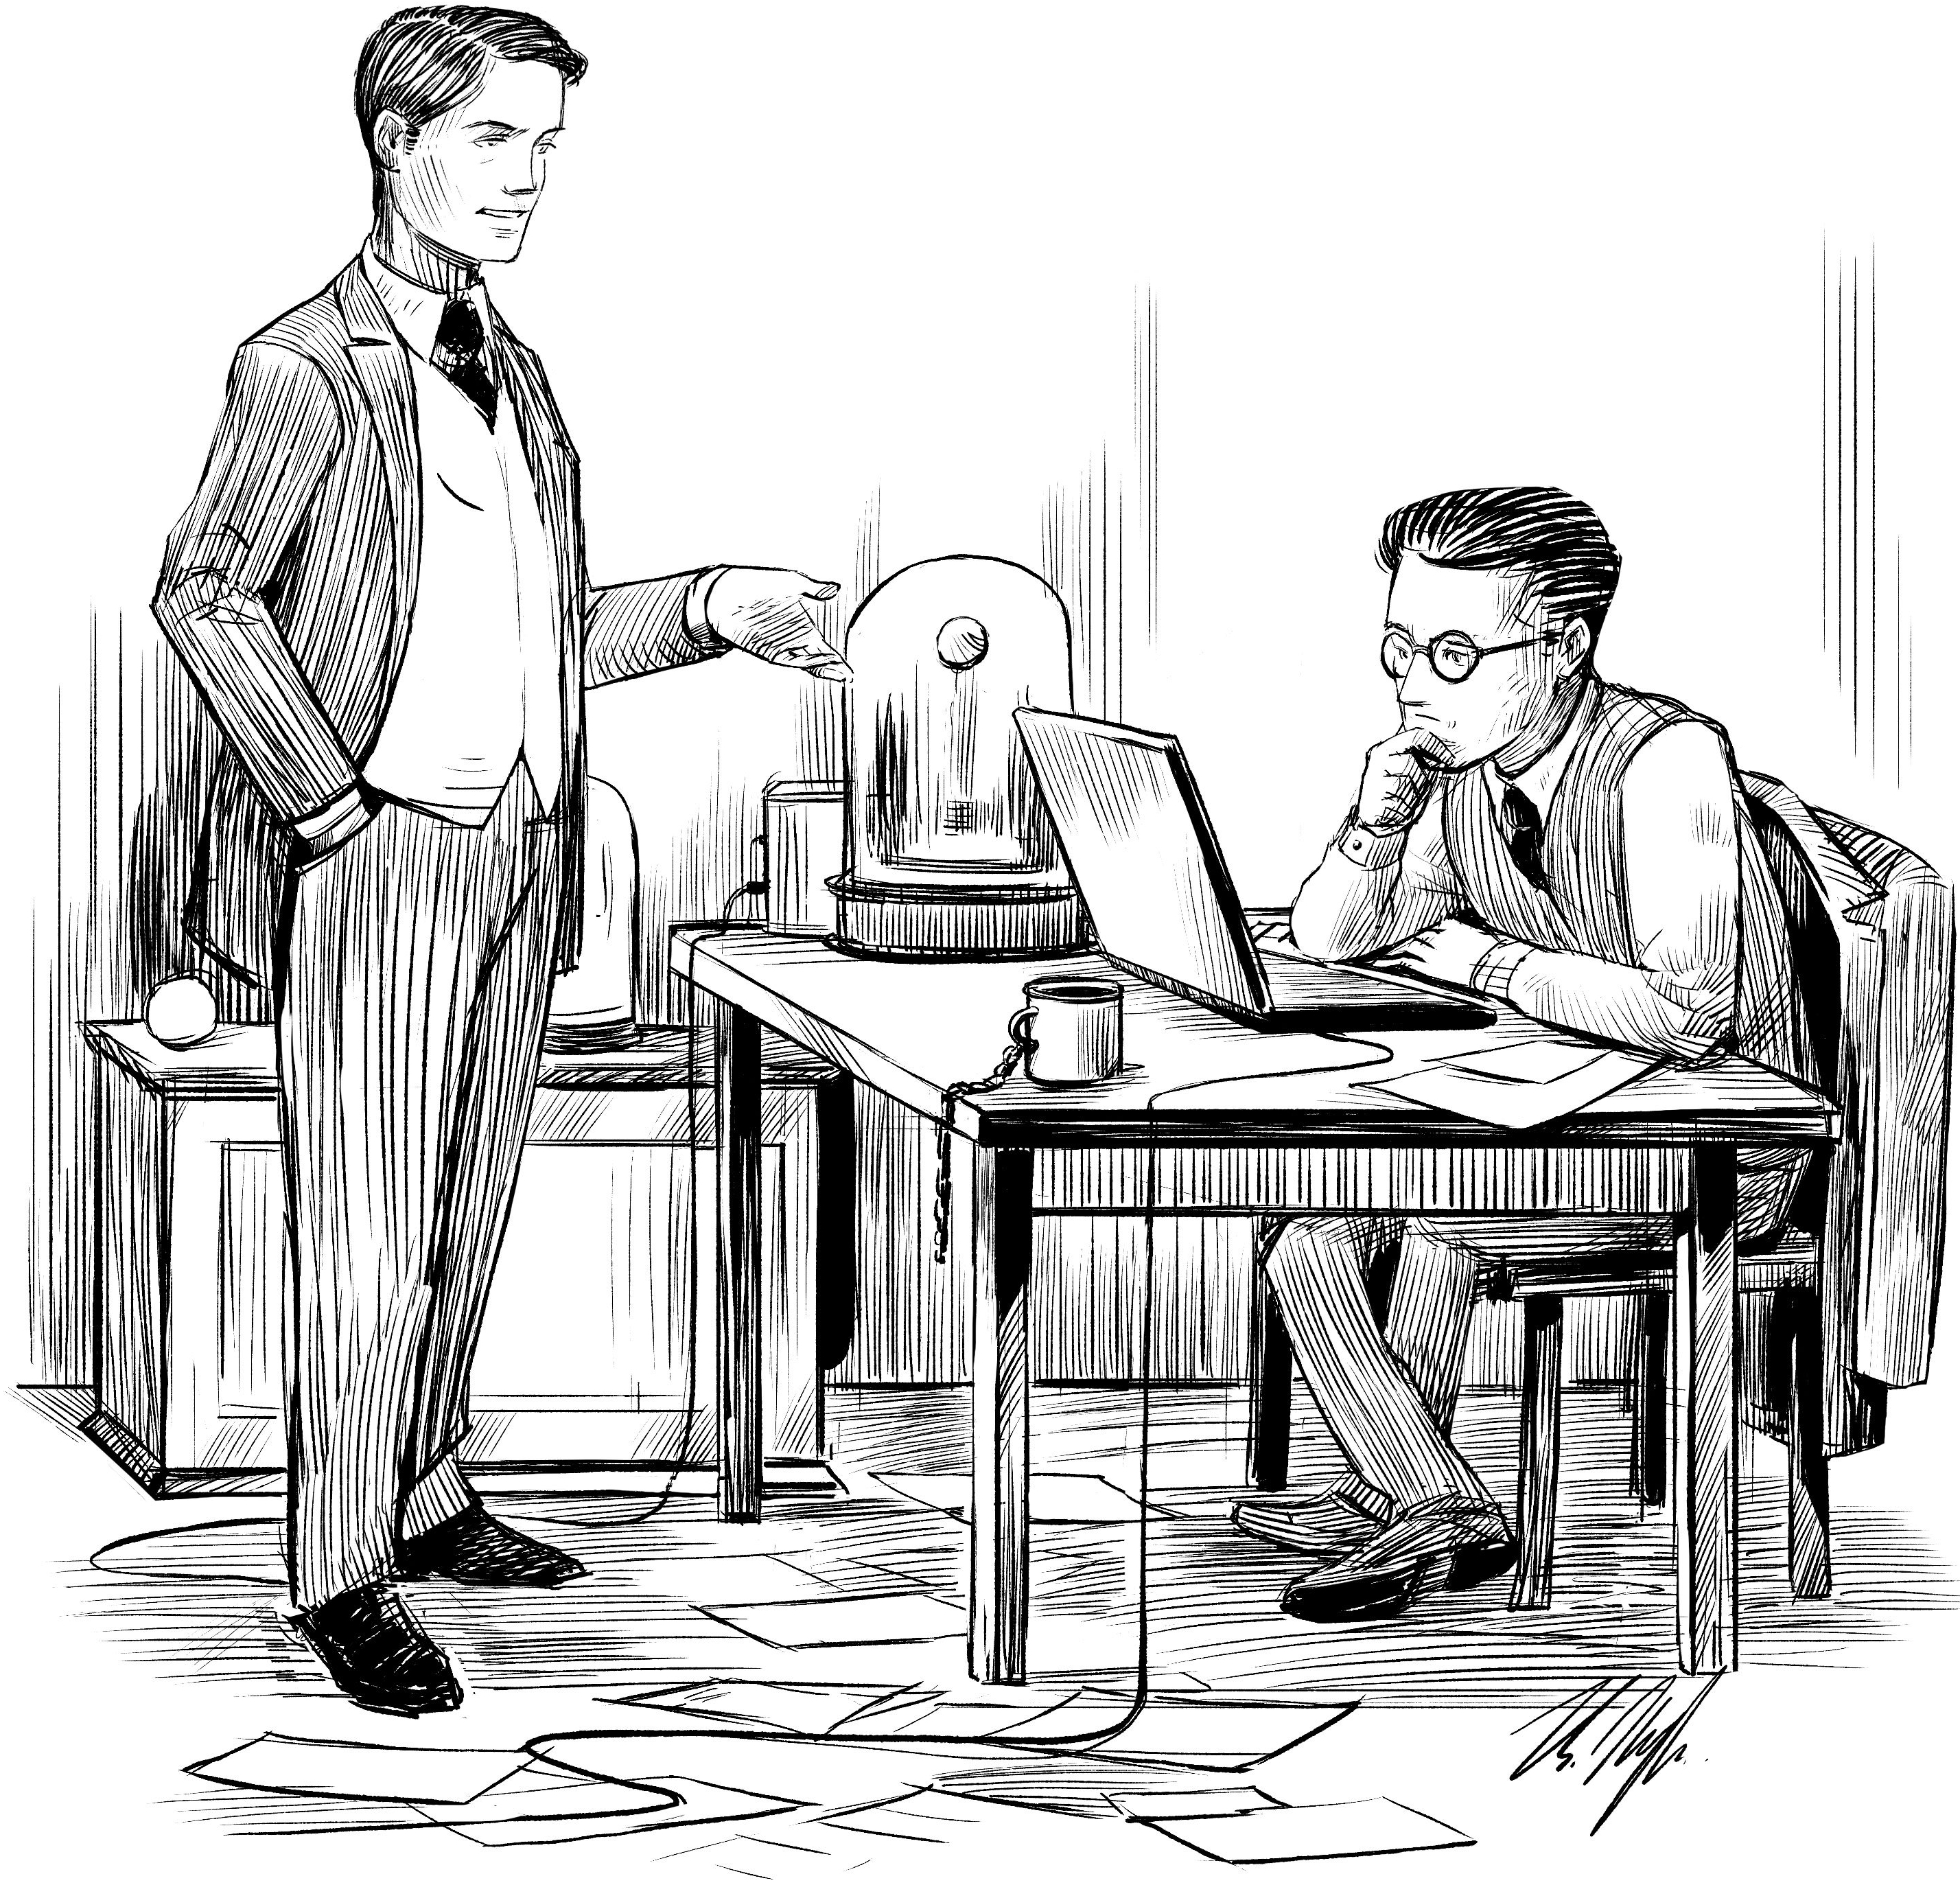
\includegraphics[scale=0.115]{cover}
\end{center}

Ever since 1931 the main protagonist in any telling of mathematical logic has always been Kurt Gödel and his First Incompleteness Theorem. Roughly speaking this theorem states that any sensible, sufficiently powerful formal system is incomplete; it'll contain a statement that is neither provable nor disprovable.

However, while the statement of the theorem is quite simple, the proof is a very different matter. Entire books, both technical and non-technical, have been devoted to it over the years. Where does this complexity come from? And what can be done about it? These are questions I already addressed in \cite{oberhoff}, though in a rather inexact manner. Indeed back then I explicitly left important details to ``smarter people'' in the conclusion. Now, some time later, and hopefully a little smarter, I want to return to the question and provide a more precise answer myself.

\section{On ``On Formally Undecidable Propositions''}

To that end let's start with a high-level overview the famous 1931 paper titled ``On Formally Undecidable Propositions Of Principia Mathematica And Related Systems'' \cite{goedel}. In this paper Gödel dealt with a formal system he had adapted from work by Bertrand Russel and Alfred North Whitehead published in three volumes of the \emph{Principia Mathematica} between 1910 and 1913. This system was based on type theory, a rather tedious framework, which has since fallen out of favor. But its salient feature---Peano Arithmetic---has survived in other systems. It defines the natural numbers and is built as follows.

\begin{definition}[Theory]
A \emph{theory} is a set of sentences closed under the inference rules of first-order logic with equality.
\end{definition}

\begin{definition}[Peano Arithmetic]
\emph{Peano Arithmetic}, or $\PA$, is the set of sentences containing these axioms:
\begin{description}
\item[Basic Peano Axioms]
\begin{description}
\item[]
\item[Zero is the first natural number:] $\forall a \colon \S a \neq 0$.
\item[Successorship is bijective:] $\forall a, b \colon \S a = \S b \leftrightarrow a = b$.
\item[Induction:] $\bigl(\mathrm{F}(0) \land \forall a \colon \mathrm{F}(a) \rightarrow \mathrm{F}(\S a)\bigr) \rightarrow \forall a \colon \mathrm{F}(a)$ for any formula $\mathrm{F}$.
\end{description}
\item[Axioms Of Arithmetic]
\begin{description}
\item[]
\item[Addition:]
\begin{align*}
\forall a \colon a + 0 & = a\\
\forall a, b \colon a + \S b & = \S(a + b)
\end{align*}
\item[Multiplication:]
\begin{align*}
\forall a \colon a \cdot 0 & = 0\\
\forall a, b \colon a \cdot \S b & = a + (a \cdot b)
\end{align*}
\end{description}
\end{description}
To this starting set we then also add any sentence that follows by the usual rules of first-order logic with equality, making Peano Arithmetic a theory.
\end{definition}

With all that in mind, here are the major steps in Gödel's 1931 proof:
\begin{description}
\item[Gödel Numbering:] Akin to modern-day ASCII encoding, Gödel first turned every formal sentence and proof into a number.
\item[Computable Enumerability:] Using the model of computation known as primitive recursive functions Gödel then implemented a proof checker in full detail, showing that $\PA$ is computably enumerable.\footnote{I am in full agreement with Robert I. Soare that ``computably enumerable'' should replace ``recursively enumerable''.}
\item[Representation:] Next, Gödel briefly pointed out that $\PA$ could represent---that is reason about---primitive recursive functions, and thereby its own proof checker.
\item[Diagonalization:] Finally, having equipped $\PA$ with the ability of introspection, Gödel diagonalized against provability-in-$\PA$. This produced a sentence asserting its own unprovability, establishing the First Incompleteness Theorem.
\end{description}

This, in essence, is still the argument given to this day. And we're not going to modify its basic structure either. Rather we'll take these items one by one and see where simplifications can be made.

\section{Gödel Numbering}

While today there is an unending variety of computational models, stretching from Diophantine equations to the specification of the Java Virtual Machine, back in 1931 there were only very few available options. That's why when Gödel drew the primitive recursive functions from the shelf the very first challenge he faced was a simple type error. His formal system $\PA$ was built out of strings over an exotic character set whereas primitive recursive functions only mapped natural numbers to natural numbers. If one wanted to devise a proof checker in this model of computation, some type conversion would be unavoidable. So that's exactly what Gödel did using a scheme that since has become known as Gödel numbering. The basic idea will be familiar to anybody who understands the concept of ASCII. Except Gödel tragically overlooked the simplicity that the humble newline character would've afforded, electing instead to encode sequences of strings (proofs) using a complicated construction involving prime numbers.

More fundamentally though---and this is a point that I really wish was made more often---it's possible to carry out the entire analysis without ever bringing up numbers at all. This is possible since, as already alluded to, Gödel could've picked any model of computation whatsoever for his proof. In particular he could've picked one which mapped strings to strings. Moreover, there's nothing standing in the way of representing such functions in Peano Arithmetic. All that's required is to reinterpret ``$0$'' as the empty string and ``$\S$'' as the lexicographical successor function. The particular choice of alphabetical ordering then becomes the only remaining vestige of Gödel's numbering scheme.

Or, to put it another way, strings already \emph{are} natural numbers.
\begin{definition}[$\mathbb{S}$]
The set of all strings is denoted $\mathbb{S}$.
\end{definition}
\[
\mathbb{S} = \{\epsilon, \text{``a''}, \text{``b''}, \dots\} = \mathbb{N}. \tag{$\epsilon$ is the empty string}
\]
All the axioms are met, so it's hard to argue otherwise. Granted, adding or multiplying strings may \emph{feel} disorienting, but surely that's only the fault of our biased upbringing.

However, as enticing as it may be to take this fully unified approach, we won't follow it to the letter here. Having the arity of our functions be strings is just a little too much. What we will do though is that we'll take our computable functions to be mappings from strings to strings. And we'll use the corner quotes usually employed to denote Gödel numbers to point directly to numerals instead.

\begin{definition}
Boldface variables denote finite sequences. E.g. $\bm{x} = x_1, \dots, x_k$.
\end{definition}

\begin{definition}[Numeral]
Let $x \in \mathbb{S}$. Then
\[
\num{x} \enskip\coloneqq\enskip \S\dots\S 0
\]
where the number of repetitions of $\S$ indicate the index of $x$ in some listing of $\mathbb{S}$. We'll call $\num{x}$ the \emph{numeral} of $x$. Also, if $\bm{x}$ is a finite sequence of strings, then $\num{\bm{x}}$ is to be taken element-wise.
\end{definition}

Of course, those that prefer the old way of looking at things are free to ignore this redefinition and stick to the conventional meaning. The proofs will read almost exactly the same.

\section{Computable Enumerability}

This section is the most notorious in Gödel's original proof. It's a chain of 46 definitions, up to 3 lines each, spread over four pages, altogether implementing a proof checker for $\PA$ using primitive recursive functions.\footnote{Gödel actually gave a relation here, not a function. But that muddles the boundary between the different sections, so I prefer to stick to functions here.} Really though, it's nothing more than an painstaking demonstration that proofs for $\PA$ could be checked by a computer. Let's state this insight more precisely.

\begin{definition}
$\cmark$ and $\xmark$ can be taken to be arbitrary strings. Their only important feature is that they're distinct.
\end{definition}

\begin{definition}[Proof Checker]
A function $\pf \colon \mathbb{S}^2 \to \{\cmark, \xmark\}$ is called a \emph{proof checker} for some theory $\T$ provided there exists an $x \in \mathbb{S}$ such that $\pf(x, \mathrm{A}) = \cmark$ if and only if $\T$ proves $\mathrm{A}$.
\end{definition}

\begin{definition}[Computably Enumerable Theory]
A theory $\T$ is considered to be \textit{computably enumerable} it has a total computable proof checker.
\end{definition}

\begin{theorem}
Peano Arithmetic is a computably enumerable theory.
\end{theorem}

\begin{prf}
Omitted.
\end{prf}

Back in 1931 mathematicians had every right to be doubtful of this claim. This was before we learned of computational universality and familiarized ourselves with higher level languages. Nowadays however this part has become just a routine programming task whose details we won't belabor.

\section{Representation}

Next, we turn to an extremely important section of the proof; the representation of computable functions as formal sentences. Roughly speaking, for a function $f$ to be represented in a theory $\T$ means that if $f(x) = y$, then $\T$ can prove this fact. And it does so by use of a single formula called the ``representation of $f$''.

\begin{definition}[Representable Function]
Let $\T$ be a theory containing the first two basic Peano axioms.\footnotemark\ Then a $k$-ary partial function $f \colon \mathbb{S}^k \to \mathbb{S}$ is said to be \emph{represented} in $\T$ if there exists a formula $\rep{f}$ with $k+1$ free variables such that whenever $f(\bm{x}) = y$ then $\T$ proves
\[
\forall b \colon \rep{f}(\num{\bm{x}}, b) \leftrightarrow b = \num{y}.
\]
(Informally this sentences states: ``$f(\bm{x})$ \emph{only} outputs $y$.'')
\end{definition}
\footnotetext{Without the first two Peano axioms we might not have any such thing as numerals in the first place.}

There are of course many kinds of functions out there which one might want to represent. But for us there's really only one kind of any consequence: the computable functions. This is enshrined by the following definition.

\begin{definition}[Turing Complete Theory]
A theory is called \emph{Turing complete} if it represents all computable functions.
\end{definition}

This terminology is more than just a passing reference to the concept of Turing complete programming languages. A Turing complete theory can quite literally be thought of as having a programming language embedded within in. And a computable function's representation is none other than its source code. This is why I chose the notation $\rep{f}$, as it's reminiscent of how the code for a Turing machine $M$ is often denoted $\langle M \rangle$. Furthermore, in order to ``execute'' a representation $\rep{f}$ on input $\bm{x}$ one can, for example, go through all possible strings and check if any of them proves a theorem of the form $\rep{f}(\num{\bm{x}}, \num{y})$ for some $y$. If so, $y$ is the output. Naturally, one would hope that this isn't the most efficient way of executing a representation. But it proves the point.

This allows us to make the central observation of this section.

\begin{theorem}
Peano Arithmetic is a Turing complete theory.
\end{theorem}

\begin{prf}
Omitted.
\end{prf}

The aforementioned result appears in many textbooks on the subject. A particularly accessible demonstration can be found in the publicly available book \textit{Incompleteness and Computability} \cite{zach}. The way I like to think of the situation is that the basic Peano axioms specify what data is. And the axioms of arithmetic delineate a universal gate set from which one can generate any computable function.  What the proof boils down to, therefore, is essentially a tedious exercise in compiler construction. As a matter of fact, even Gödel himself only sketched this part of the argument in his 1931 paper, expounding the details in lectures given in 1934.\footnote{These lectures were attended by Alonzo Church's graduate students Stephen C. Kleene and John B. Rosser. Together they took notes which were first distributed via mimeograph until they were published in 1965 in an anthology by Martin Davis \cite{davis}.}

In broad strokes, one first takes the high-level language used in the rest of the argument---or at least some model of computation one trusts to be universal---and translates it down to a model of computation chosen to be as convenient as possible for Peano Arithmetic to represent. Then one systematically converts every function definable in the chosen model into a formula obeying the definition of representability.

Admittedly, this does open us up to the charge that we're not simplifying much at all over the course of this presentation. We're just moving all the nasty parts out of sight. But I disagree. I think there's real clarity to be won by using the definition for Turing completeness to impose a clean interface. And in the upcoming section I hope to show that.

\section{Diagonalization}

Enough with the omissions! Let's actually prove something.

\subsection{Setup}

\begin{definition}[Pseudo-Term]
Let $f$ be a representable function. Then the expression $f(\bm{a})$ is referred to as a \emph{pseudo-term} or \emph{p-term}. And for an expression of the form $\mathrm{F}(f(\bm{a}))$ we define
\[
\mathrm{F}(f(\bm{a})) \enskip\coloneqq\enskip \exists b \colon \rep{f}(\bm{a}, b) \land \mathrm{F}(b).
\]
\end{definition}

Some remarks are in order.
\begin{itemize}
\item $\bm{a}$ in the definition above is a free formal variable, used as a stand-in. 

\item As can easily be checked, multiple simultaneous occurrences of this notation expand equivalently, no matter the order of expansion---not that this'll come up for us anyways.

\item If $\mathrm{F}(f(\bm{a}))$ appears nested in some larger formula, then we still only ``pull out'' $f(\bm{a})$ from $\mathrm{F}$, not the entire formula.

\item Two important special cases are $f(\bm{a}) = b$ and $f(\bm{a}) \neq b$. The former expands to $\exists c \colon \rep{f}(\bm{a}, c) \land c = b$ which is obviously logically equivalent to $\rep{f}(\bm{a}, b)$. And the latter is meant to become $\neg(f(\bm{a}) = b)$ and then $\neg \exists c \colon \rep{f}(\bm{a}, c) \land c = b$ which is the equivalent of $\neg\rep{f}(\bm{a}, b)$.
\end{itemize}

\begin{lemma}\label{lm-1}
Let $f$ be represented in $\T$. And assume that $f(\bm{x}) = y \neq z$. Then $\T$ proves
\[
f(\num{\bm{x}}) = \num{y} \quad\text{and}\quad f(\num{\bm{x}}) \neq \num{z}.
\]
\end{lemma}

\begin{prf}
Clearly, the first two Peano axioms suffice to prove $\num{y} = \num{y}$ and $\num{z} \neq \num{y}$. And by representability $\T$ proves $\forall b \colon f(\num{\bm{x}}) = b \leftrightarrow b = \num{y}$. Thus, instantiating $b$ once as $\num{y}$ and once as $\num{z}$ plus simple logic gives us what we want.
\end{prf}

\begin{lemma}\label{lm-2}
Let $f$ be represented in $\T$. And suppose $f(\bm{x}) = y$. Then $\T$ proves $\mathrm{F}(f(\num{\bm{x}})) \leftrightarrow \mathrm{F}(\num{y})$ for any formula $\mathrm{F}$.
\end{lemma}

\begin{prf}
In the forward direction $\mathrm{F}(f(\num{\bm{x}}))$ translates to $\exists b \colon f(\num{\bm{x}}) = b \land \mathrm{F}(b)$. This easily combines with the provable sentence $\forall b \colon f(\num{\bm{x}}) = b \leftrightarrow b = \num{y}$ to give $\mathrm{F}(\num{y})$.

And in the other direction $f(\num{\bm{x}}) = \num{y}$ given to us by Lemma \ref{lm-1} together with $\mathrm{F}(\num{y})$ yields $\exists b \colon f(\num{\bm{x}}) = b \land \mathrm{F}(b)$.
\end{prf}

\begin{definition}
Writing $A(\rep{f})$ in the signature of an algorithm $A$ means that $A$ expects a representation as input, akin to pattern matching. For invalid inputs (which we'll avoid) the algorithm is allowed to arbitrarily misbehave.
\end{definition}

\begin{lemma}[Diagonal Lemma]
Let $\T$ be a Turing complete theory. And let $\mathrm{P}$ be a predicate. Then there exists a sentence $\mathrm{A}$ referred to as a ``fixed point'' such that $\T$ proves $\mathrm{A} \leftrightarrow \mathrm{P}(\num{\mathrm{A}})$.
\end{lemma}

\begin{prf}
Consider the following algorithm.
\begin{algo}
\Function{$D(\rep{f})$}{}
  \State\Return $\mathrm{P}(f(\numrep{f}))$
\EndFunction
\end{algo}
Then $D(\rep{D}) = \mathrm{P}(D(\numrep{D}))$. So $\T$ proves $\mathrm{P}(D(\numrep{D})) \leftrightarrow \mathrm{P}(\num{\mathrm{P}(D(\numrep{D}))\!})$ by Lemma \ref{lm-2}, making $\mathrm{P}(D(\numrep{D}))$ a fixed point.
\end{prf}

\subsection{The First Incompleteness Theorem}

The main use of the Diagonal Lemma is to produce the Gödel sentence. Consider the predicate
\begin{definition}[$\Pvb_\mathfrak{G}$]
\hspace{2.85cm} $\Pvb_{\mathfrak{G}}(a) \enskip\coloneqq\enskip \exists b \colon \pf(b,a) = \num{\cmark}$
\end{definition}
where $\pf$ is the proof checker Gödel originally constructed. Then if one applies the Diagonal Lemma to $\neg \Pvb_{\mathfrak{G}}$, one produces a sentence $\mathrm{G}$ such that $\PA$ proves $\mathrm{G} \leftrightarrow \neg\Pvb_{\mathfrak{G}}(\num{\mathrm{G}})$. Informally this sentence states: ``I am not provable.'' which, assuming that $\PA$ is consistent, turns out to be true. Furthermore, one can also show that $\neg \mathrm{G}$ can't be provable either. Though this needs the stronger assumption that $\PA$ is \emph{correct}; if $\PA$ proves something, then it is actually so. Or at least it requires $\omega$-consistency; if $\PA$ proves that some unbounded search terminates, then it actually does. So in summary, if $\PA$ is $\omega$-consistent, it is incomplete.

For the audience in 1931 this already settled the matter. Still, in 1936 John B. Rosser found a way to iron out the last wrinkle as well by using the following predicate instead \cite{rosser}.
\begin{definition}[$\bm{<}$]
We define
\[
a < b \enskip\coloneqq\enskip \exists c \colon a + c = b.
\]
and, as a convenience, for any formula $\mathrm{F}$
\[
\forall a < b \colon F(a,b) \enskip\coloneqq\enskip \forall a \colon a < b \rightarrow F(a,b).
\]
\end{definition}

\begin{definition}[$\bm{\mathit{neg}}$]
$\ng$ is the (computable) function which attaches ``$\neg$'' to the front of its input.
\end{definition}

\begin{definition}[$\Pvb_{\mathfrak{R}}$]
\hspace{0.85cm}$\Pvb_{\mathfrak{R}}(a) \enskip\coloneqq\enskip \exists b \colon \pf(b,a) = \num{\cmark} \land \forall c < b \colon \pf(c,\ng(a)) \neq \num{\cmark}$
\end{definition}
If one applies the Diagonal Lemma to $\neg\Pvb_{\mathfrak{R}}$, it produces the Rosser sentence $\mathrm{R}$ which can be paraphrased as: ``For every proof of me there exists a shorter disproof.'' This sentence, unlike $\mathrm{G}$, can be demonstrated to be neither provable nor disprovable assuming only the consistency of $\PA$ , giving us the much nicer formulation: if $\PA$ is consistent, it is incomplete.

Spelling all of this out and checking the details takes a bit of work though. For instance, the probably most famous exposition of the First Incompleteness Theorem in \textit{Gödel, Escher, Bach} takes about ten pages (not counting a dialogue) to make it from the observation that $\PA$ can represent all computable functions at the end of chapter thirteen to Gödel's weaker version of the First Incompleteness Theorem. Also Rosser's improvement typically invokes the fact that $\PA$ can prove $\forall a < \S n \colon \mathrm{F}(a) \leftrightarrow \bigwedge_{a=0}^n \mathrm{F}(a)$ for any formula $\mathrm{F}$ and numeral $n$. This brings us then to another way of proving the First Incompleteness Theorem which, in my mind, fully captures the essence while being much, much leaner.

\begin{theorem}[First Incompleteness Theorem]\label{tm-first}
Let $\T$ be a consistent, computably enumerable, and Turing complete theory. Then $\T$ is incomplete.
\end{theorem}

\begin{prf}
First, we construct the following algorithm.
\begin{algo}
\Function{$Z(\rep{f})$}{}
  \For{$x \in \mathbb{S}$}
    \If{$x$ proves $f(\numrep{f}) \neq \num{\cmark}$}
      \State\Return \hspace{-1.8pt} $\cmark$
    \EndIf
    \vspace{-2.75pt}
    \If{$x$ proves $f(\numrep{f}) = \num{\cmark}$}
      \State\Return \hspace{-1.8pt} $\xmark$
    \EndIf
  \EndFor
\EndFunction
\end{algo}
This lets us produce
\[
\mathrm{R} \enskip\coloneqq\enskip Z(\numrep{Z}) \neq \num{\cmark}.
\]
Now suppose that $\mathrm{R}$ was decidable. Then there must exist a \emph{first} $x \in \mathbb{S}$ which decides $\mathrm{R}$. This leads to two cases.
\newline
\begin{minipage}{0.5\textwidth}
\smallskip
\begin{description}[leftmargin=0.5cm]
\item[Suppose $x$ proves $\mathrm{R}$:]
\begin{itemize}[label={$\Rightarrow$}]
\item[]
\item $Z(\rep{Z})$ returns $\cmark$ upon finding $x$.
\item $\T$ proves $\neg \mathrm{R}$ by Lemma \ref{lm-1}, an inconsistency.
\end{itemize}
\end{description}
\end{minipage}
\begin{minipage}{0.5\textwidth}
\smallskip
\begin{description}[leftmargin=0.5cm]
\item[Suppose $x$ proves $\neg \mathrm{R}$:]
\begin{itemize}[label={$\Rightarrow$}]
\item[]
\item $Z(\rep{Z})$ returns $\xmark$ upon finding $x$.
\item $\T$ proves $\mathrm{R}$ by Lemma \ref{lm-1}, an inconsistency.\qedhere
\end{itemize}
\end{description}
\end{minipage}
\end{prf}

The sentence $\mathrm{R}$ used in the above proof carries its name for a reason. It's because, as some reflection will reveal, $\mathrm{R}$ is none other than the Rosser sentence, claiming: ``For every proof of me there exists a shorter disproof.'' Also, in order to recover the original ``I am not provable'' one only needs to drop the last two lines of $Z$.

We also get the following important corollary.

\begin{corollary}
If $\PA$ is consistent, it is incomplete.
\end{corollary}

\begin{prf}
We've already seen that $\PA$ is computably enumerable and Turing complete. So if we add in the assumption of consistency the First Incompleteness Theorem tells us that $\PA$ is incomplete.
\end{prf}

\section{The Second Incompleteness Theorem}

At a high level the Second Incompleteness Theorem isn't all that hard to grasp. We've already seen that if $\PA$ is consistent, then $\mathrm{G}$ isn't provable and thereby true. In short, $\Con \rightarrow \mathrm{G}$ where $\Con$ expresses the consistency of $\PA$. What's more, as Gödel first noted in 1931, this fact can be proven by $\PA$ as well since it can step through the proof of the First Incompleteness Theorem just the same. But that means that if $\PA$ could prove $\Con$, then $\PA$ could also prove $\mathrm{G}$ by modus ponens which is impossible. Whence the Second Incompleteness Theorem: if $\PA$ is consistent, then it can't prove this to be so.

Alas, the crucial fact that $\Con \rightarrow \mathrm{G}$ can be proven in $\PA$ is notoriously difficult to establish rigorously. Gödel himself famously concluded his 1931 paper stating: ``The results will be stated and proved in fuller generality in a forthcoming sequel. There too, the mere outline proof we have given of [the Second Incompleteness Theorem] will be presented in detail.'' Such a sequel never came. Instead, the first rigorous demonstration appeared in 1939 in the second volume of \textit{Foundations of Mathematics} written by David Hilbert and his assistant Paul Bernays---Bernays being the main author.

But besides technical issues, there are also philosophical ones. Most importantly, what exact expression should we choose for $\Con$? Gödel had the obvious in mind:
\begin{definition}[$\Con_{\mathfrak{G}}$]
\hspace{2.25cm}$\Con_{\mathfrak{G}} \enskip\coloneqq\enskip \neg \exists a \colon \Pvb_{\mathfrak{G}}(a) \land \Pvb_{\mathfrak{G}}(\ng(a))$
\end{definition}
However, Gödel had many freedoms when making his construction. What made the choice he arrived at the correct one? This question is brought to a head when one examines alternative derived from Rosser's predicate.
\begin{definition}[$\Con_{\mathfrak{R}}$]
\hspace{2.25cm}$\Con_{\mathfrak{R}} \enskip\coloneqq\enskip \neg \exists a \colon \Pvb_{\mathfrak{R}}(a) \land \Pvb_{\mathfrak{R}}(\ng(a))$
\end{definition}
If one were to use this consistency statement instead, then $\PA$ actually \emph{could} prove its own consistency. This happens for the simple reason that \emph{every} theory, whether consistent or not, is ``consistent'' according to the Rosser definition.

To answer all this history eventually decided to put down three conditions that any provability predicate should meet.

\begin{definition}[Provability Predicate]
A predicate $\Pvb$ is considered a \emph{provability predicate} for a theory $\T$ if it obeys the following three derivability conditions for any sentences $\mathrm{A}, \mathrm{B}$:
\begin{description}
\item[(D1)] If $\T$ proves $\mathrm{A}$, then $\T$ proves $\Pvb(\num{\mathrm{A}})$.
\item[(D2)] $\T$ proves $\Pvb(\num{\mathrm{A}}) \rightarrow \Pvb(\num{\Pvb(\num{\mathrm{A}})})$.
\item[(D3)] $\T$ proves $\Pvb(\num{\mathrm{A}}) \land \Pvb(\num{\mathrm{A} \rightarrow \mathrm{B}}) \rightarrow \Pvb(\num{\mathrm{B}})$.
\end{description}
\end{definition}

From these three conditions---also known as the HBL-derivability conditions (Hilbert, Bernays, Löb)---the Second Incompleteness Theorem can be derived in short order. This both shuts the door on Rosser's predicate and provides a convenient layer of abstraction, similar to representability.

The only question left on the table is then: does some proposed provability predicate actually meet the criteria? This is where all the fearsome details end up hiding; details into which we won't delve much further. Because instead I want to showcase an alternative pathway towards an intriguing ``Little Second Incompleteness Theorem'' which is much easier to prove. It only requires a small act of insanity.

We begin with a predicate $\Pvb$ that obeys (D1) and use it to construct a fixed point of $\neg \Pvb$; Gödel's $\mathrm{G}$ for example. Then we add a small wrapper to $\Pvb$ which by default simply calls through to $\Pvb$. Except, when it encounters the negated fixed point the wrapper first chops off the negation.

\begin{lemma}\label{lm-U}
Let $\T$ be a Turing complete theory. Let $\Pvb$ be a predicate obeying (D1) ($\Pvb_{\mathfrak{G}}$ or $\Pvb_{\mathfrak{R}}$ will do equally well). And let $\mathrm{G}$ be a Gödel sentence for $\Pvb$ such that $\T$ proves $\mathrm{G} \leftrightarrow \neg \Pvb(\num{\mathrm{G}})$. Then there exists a predicate $\Pvb'$ such that:
\begin{description}
\item[(DG)] $\T$ proves $\mathrm{G} \leftrightarrow \neg\Pvb'(\num{\mathrm{G}}) \leftrightarrow \neg\Pvb'(\num{\neg \mathrm{G}})$
\item[(D1)] If $\T$ proves $\mathrm{A}$, then $\T$ proves $\Pvb'(\num{\mathrm{A}})$ for every sentence $\mathrm{A}$.
\end{description}
\end{lemma}

\begin{prf}
We start with the following ``filter'' algorithm.

\begin{algo}
\Function{$\ft(\mathrm{A})$}{}
  \If{$\mathrm{A}$ is equal to $\neg \mathrm{G}$}
    \State\Return $\mathrm{G}$
  \EndIf
  \State\Return $\mathrm{A}$
\EndFunction
\end{algo}
And our ``provability predicate'':
\[
\Pvb'(a) \enskip\coloneqq\enskip \Pvb(\ft(a)).
\]

\begin{description}
\item[(DG):] By definition $\neg\Pvb'(\num{\mathrm{G}})$ and $\neg\Pvb'(\num{\neg \mathrm{G}})$ are respectively equal to $\neg\Pvb(\ft(\num{\mathrm{G}}))$ and $\neg\Pvb(\ft(\num{\neg \mathrm{G}}))$. And since $\ft$ outputs $\mathrm{G}$ on both of these inputs we can use Lemma \ref{lm-2} to prove both of these sentences equivalent to $\neg\Pvb(\num{\mathrm{G}})$. We already know that $\neg\Pvb(\num{\mathrm{G}})$ is equivalent to $\mathrm{G}$. Therefore,
\[
\mathrm{G} \leftrightarrow \neg\Pvb'(\num{\mathrm{G}}) \leftrightarrow \neg\Pvb'(\num{\neg \mathrm{G}}).
\]

\item[(D1):] If $\mathrm{A} = \neg \mathrm{G}$, then we've just seen that $\neg \mathrm{G} \leftrightarrow \Pvb'(\num{\neg \mathrm{G}})$. So if $\mathrm{A}$ is provable, $\Pvb'(\num{\mathrm{A}})$ is too.

Otherwise, if $\mathrm{A} \neq \neg \mathrm{G}$, then $\ft(\mathrm{A}) = \mathrm{A}$. So by Lemma \ref{lm-2} we have $\Pvb'(\num{\mathrm{A}}) \leftrightarrow \Pvb(\num{\mathrm{A}})$; the right-hand side being provable because we assume that $\Pvb$ already obeys (D1).\qedhere
\end{description}
\end{prf}

\begin{theorem}[Little Second Incompleteness Theorem]
Let $\T$ be a consistent, computably enumerable, and Turing complete theory. Then the consistency statement
\[
\Con' \enskip\coloneqq\enskip \neg \exists a \colon \Pvb'(a) \land \Pvb'(\ng(a))
\]
where $\Pvb'$ is constructed as in Lemma \ref{lm-U} is not provable in $\T$.
\end{theorem}

\begin{prf}
Through (DG) and an application of Lemma \ref{lm-2} for the $\ng$ function we easily get
\[
\neg \mathrm{G} \rightarrow \Pvb'(\num{\mathrm{G}}) \land \Pvb'(\num{\neg \mathrm{G}}) \qquad\text{and}\qquad \Pvb'(\num{\mathrm{G}}) \land \Pvb'(\num{\neg \mathrm{G}}) \rightarrow \neg\Con'.
\]
Thus, if $\Con'$ were provable, then by the converse $\mathrm{G}$ is too. This makes $\Pvb'(\num{\mathrm{G}})$ provable by condition (D1). However, by equivalency that would prove $\neg \mathrm{G}$ as well, leaving $\T$ inconsistent.
\end{prf}

We've certainly shown \emph{some} sentence to be unprovable here. But, remembering how we've messed with the initial predicate, why should we still treat $\Con'$ seriously as an expression of consistency? Let me explain.

Take $\Pvb_{\mathfrak{G}}$ as an example. Then by construction we have $\neg \mathrm{G} \leftrightarrow \Pvb_{\mathfrak{G}}(\num{\mathrm{G}})$. Therefore, $\Pvb_{\mathfrak{G}}(\num{\neg\mathrm{G}})$ is essentially the same as $\Pvb_{\mathfrak{G}}(\num{\Pvb_{\mathfrak{G}}(\num{\mathrm{G}})})$. Indeed, if we look back at how $\mathrm{G}$ is constructed in the Diagonal Lemma, these sentences are related even at a syntactical level. What we're asking the predicate here is: ``How would you answer the question: ``Is $\mathrm{G}$ provable?''?'' And all our modification is doing when it tosses the negation symbol is to simplify the question down to: ``Is $\mathrm{G}$ provable?'' From a human perspective this seems entirely reasonable. After all, would any of \emph{us} when asked ``How would you answer the question: ``What's $2+2$?''?'' actually go through the whole process of simulating our own brain as it ponders $2+2$? Not me. I just answer: ``$4$.'' $\Pvb'$ merely takes that exact same mental shortcut for a single judiciously chosen question. And since $\mathrm{G}$ is unprovable, we know that this is a fool's errand anyway.

Naturally, there's a catch here. And it's this. If we imagine writing $\Con_{\mathfrak{G}}$ as an infinite conjunction, it would look something like the following.
\[
\Con_{\mathfrak{G}} \enskip=\enskip \bigl(\neg\Pvb_{\mathfrak{G}}(0) \lor \neg\Pvb_{\mathfrak{G}}(\ng(0))\bigr) \land \cdots \land \bigl(\neg\Pvb_{\mathfrak{G}}(\num{\mathrm{G}}) \lor \neg\Pvb_{\mathfrak{G}}(\num{\neg\mathrm{G}})\bigr) \land \cdots
\]
All of these terms appear in $\Con_{\mathfrak{G}}'$ in completely equivalent form, the only exception being $\neg\Pvb_{\mathfrak{G}}(\num{\mathrm{G}}) \lor \neg\Pvb_{\mathfrak{G}}(\num{\neg\mathrm{G}})$ where we instead encounter the equivalent of only $\neg\Pvb_{\mathfrak{G}}(\num{\mathrm{G}})$. Thus $\Con_{\mathfrak{G}}' \rightarrow \Con_{\mathfrak{G}}$ by a hair's width. And in the other direction $\Con_{\mathfrak{G}} \rightarrow \Con_{\mathfrak{G}}'$ as well. We just need $\Con_{\mathfrak{G}} \rightarrow \mathrm{G}$, a detail which will be stated and proved in fuller generality in a forthcoming sequel.\footnote{Or maybe not.}

\section{A Hierarchy Theorem}

Up to this point we've mostly been retreading the beaten path. Next up, I also want to broaden our horizons a little by looking at some more novel connections to complexity theory. Truth be told, this section was the original motivation for writing all of this. I just couldn't bring myself to beeline straight to this point without filling in the bigger picture.

The thing is, similarities between the First Incompleteness Theorem and the Halting Problem have long been noted. But looking at our simplified proof of the Incompleteness Theorem they stand out more than ever. The Halting problem is proven undecidable by running a certain program on its own source code. And the First Incompleteness Theorem follows from running a very similar program on its own representation.

This might bring to mind then that the Halting Problem was famously modified by Juris Hartmanis and Richard E. Stearns in 1965 in order to establish the Time Hierarchy Theorem \cite{time-hierarchy}. A question thus arises: can the same modification be performed on the First Incompleteness Theorem? And if so, what is the outcome? The answer is yes, an analogue of the Nondeterministic Time Hierarchy Theorem, originating from Stephen A. Cook \cite{cook}, can be proven along these lines. Here's how.

To start with we're going to have to be more restrictive as to what constitutes a proof. Mere computable enumerability doesn't cut it anymore.

\begin{definition}[Proof]
Let $\T$ be a theory. We'll consider a string $x \in \mathbb{S}$ to be a proof of $\mathrm{A} \in \T$ if:
\begin{itemize}
\item Each line of $x$ (when separating by some newline character) is either an axiom of $\T$ or follows from the previous lines by an inference rule of first-order logic.
\item The last line of $x$ is $\mathrm{A}$.
\end{itemize}
\end{definition}

We'll also need to define the analogue of a computational problem.

\begin{definition}
The length of a string $x \in \mathbb{S}$ is denoted $\lvert x \rvert$.
\end{definition}

\begin{definition}[Proof Problem]
Fix a theory $\T$. Then any set of sentences $\mathbf{A}$ will be considered a \emph{proof problem}. Furthermore, the \textit{(proof) complexity} $f$ of $\mathbf{A}$ is defined to be
\[
f(n) \coloneqq \max_{\substack{\mathrm{A} \in \mathbf{A} \colon\\ \lvert \mathrm{A} \rvert \leq n}} \; \min_{\substack{x \in \mathbb{S} \colon\\ x \text{ decides } \mathrm{A}}} \lvert x \rvert
\]
Informally, it's the minimum number of symbols required to decide every sentence up to length $n$. Also, if $\mathbf{A}$ contains an undecidable sentence, then we refer to $\mathbf{A}$ as \emph{undecidable} instead.
\end{definition}

Onto the result.

\begin{theorem}[Proof Hierarchy Theorem]
Let $\T$ be a consistent, computably enumerable, and Turing complete theory. Let $g$ be computable, monotone, and $g(n) = \Omega(n)$. And let $f(n+1) = o(g(n))$. Then there exists a proof problem with complexity $O(g(n))$ but not $O(f(n))$.
\end{theorem}

\begin{prf}
Consider the following algorithm.
\begin{algo}
\Function{$Z_g(\rep{f}, s)$}{}
  \State $m \gets \bigl\lvert f(\numrep{f}, \num{s}) = \num{\cmark}\bigr\rvert$
  \For{$x\in\mathbb{S} : \lvert x \rvert \leq g(m)$}
    \If{$x$ proves $f(\numrep{f}, \num{s}) \neq \num{\cmark}$}
      \State\Return $\cmark$
    \EndIf
    \If{$x$ proves $f(\numrep{f}, \num{s}) = \num{\cmark}$}
      \State\Return $\xmark$
    \EndIf
  \EndFor
  \State\Return $\cmark$
\EndFunction
\end{algo}
This gives rise to the proof problem
\[
\mathbf{B} = \Bigl\{Z_g(\numrep{Z_g}, \num{s}) = \num{\cmark} : s \in \mathbb{S} \Bigr\}
\]
where the $s$ just serves to turn our single undecidable sentence from the First Incompleteness Theorem into an infinitely large family.

To start with, $\mathbf{B}$ can't have complexity $g(m)$ by reasoning exactly as in the First Incompleteness Theorem. Any proofs this short would be found by $Z_g$ and swiftly lead to an inconsistency. That means however that \emph{eventually} $Z_g$ will arrive at its last line and output $\cmark$. By the definition of representability that makes every sentence in $\mathbf{B}$ provable and gives this problem a well defined proof complexity $h$ such that $g(m) < h(m)$.

Now define
\[
\mathbf{A} = \Bigl\{ \mathrm{B} \land \S \dots \S 0 \neq 0 : \mathrm{B} \in \mathbf{B},\; n = g^{-1}(h(m)) \Bigr\}
\]
where $m$ is the length of the original sentence $\mathrm{B}$, $n$ is the length of the new sentence, and $g^{-1}(j) \coloneqq \argmin_i j \leq g(i)$. The aim here is to dilute the sentences in $\mathbf{B}$ with padding until we reach complexity $O(g(n))$ and no lower.

First, let's verify that $\mathbf{A}$ has proof complexity $O(g(n))$. To that end note that $i \leq g(g^{-1}(i))$ for any $i \in \mathbb{N}$. So we can say that it takes $h(m) \leq g(g^{-1}(h(m))) = g(n)$ symbols to prove $\mathrm{B}$. And it takes $O(n)$ symbols to prove the padding. Since $g$ is monotone and $g(n) = \Omega(n)$ this gives us proofs of length $O(g(n))$ overall.

And second, we need to rule out $O(f(n))$ as a proof complexity for $\mathbf{A}$. This time, opposite to the previous case, note that $g(g^{-1}(i) - 1) < i$ for any $i \in \mathbb{N}$. Hence,
\[
O(f(n)) = o(g(n-1)) = o(g(g^{-1}(h(m))-1)) = o(h(m)).
\]
This leads us to conclude that if $\mathbf{A}$ and thereby $\mathbf{B}$ had proofs of length $O(f(n))$, then it would have proofs of length $o(h(m))$. But that contradicts the assumption that $h(m)$ denoted the length of the shortest proofs for $\mathbf{B}$.
\end{prf}

As already mentioned, this theorem is quite similar to the Nondeterministic Time Hierarchy. Here's a reminder.

\begin{theorem}[Nondeterministic Time Hierarchy Theorem]
Let $g$ be time constructible (one can compute $g(n)$ in $O(g(n))$ steps). And let $f(n+1) = o(g(n))$. Then $\mathsf{NTIME}(f(n)) \subsetneq \mathsf{NTIME}(g(n))$.
\end{theorem}

\begin{prf}
Omitted.
\end{prf}

There are a couple of lines along which I'd like to compare these theorems.

\begin{itemize}
\item Fascinatingly, even though the proof of the Proof Hierarchy Theorem runs along very different lines than the proof of the Nondeterministic Time Hierarchy Theorem (at least the one I'm familiar with by \v{Z}ák Stanislav \cite{stanislav}), the exact same $+1$ shows up in the formulation.
\item Whereas the Nondeterministic Time Hierarchy Theorem requires $g$ to be time constructible, the Proof Hierarchy Theorem is already satisfied with mere computability.
\item The Proof Hierarchy Theorem doesn't make any demands regarding the computational complexity of checking proofs. In particular checking whether a given sentence is an axiom might be arbitrarily difficult.
\item Fundamentally, the nondeterminstic time hierarchy is a hierarchy \emph{among} verifiers, while the proof hierarchy is a hierarchy among the inputs for a \emph{fixed} verifier.
\item The main sticky point that prevents this proof from being turned into a simpler demonstration of the Nondeterministic Time Hierarchy Theorem is that, as Manuel Blum demonstrated \cite{blum}, computational problems might not have a \emph{minimum} complexity $h$.
\end{itemize}

\section{Oracles}

Last but not least, I want to take a brief look at a topic near and dear to computer scientists of the present: oracles. This section was born from the following line of thought.

Take Peano Arithmetic and add a set of uncomputable axioms to it. The simplest example would be an axiomatization of the Halting Problem by means of a predicate $\mathrm{H}$ so that either $\mathrm{H}(\num{x})$ or $\neg\mathrm{H}(\num{x})$ is an axiom depending on whether or not $x$ describes a halting computation. Such a predicate can already be defined in the language of arithmetic. This theory, call it $\PA+\mathrm{H}$, is no longer computably enumerable so the First Incompleteness Theorem won't apply anymore. The step that breaks in the proof is that the algorithm $Z$ we constructed now needs to run an uncomputable proof checker as a subroutine. Sure, we could make $Z$ ``computable'' if we gave it access to an oracle for the Halting Problem. But then we still face the challenge of representing $Z$. We only know how to represent computable functions, not functions that call on a Halting Problem oracle. To represent such functions it seems that we'd also need a way to represent the Halting Problem. Except, that is precisely what $\PA+\mathrm{H}$ conveniently provides for us!

To turn this idea into a proof we're going to need a lemma. Simply put, if our theory is Turing complete and can also represent some oracle, then it should be possible to represent algorithms which call said oracle. The strategy to prove this lemma is straightforward. We chop the computation up into computable sections and oracle queries. And then we prove that the input of each section determines the input of the next, ultimately determining the output of the function. One detail worth pointing out: for the computable sections to be able to predict the next query requires that they know the whole history of oracle responses. This means if our responses are $r_1, \dots, r_k$, then we'll sequentially feed our computable sections lists of the form $(), (r_1), (r_1, r_2), \dots, (r_1, \dots, r_k)$.

There's just one blemish. Namely we're also going to need the following fact which we were able to avoid in our earlier proof of the First Incompleteness Theorem.

\begin{lemma}\label{lm-5}
$\PA$ proves
\[
\forall a < \S n \colon \mathrm{F}(a) \enskip\leftrightarrow\enskip \bigwedge_{a=0}^n \mathrm{F}(a)
\]
for any formula $\mathrm{F}$ and numeral $n$.
\end{lemma}

\begin{prf}
Omitted.
\end{prf}

This lemma is quite standard. For example, it appears as lemma 4.23 in \textit{Incompleteness and Computability} \cite{zach} where it is shown for the fragment of $\PA$ called Robinson Arithmetic, or $\mathbf{Q}$. However, it doesn't appear to follow from mere Turing completeness. Nor did I find a particularly elegant auxiliary assumption to combine with Turing completeness which would've yielded this fact. So for the moment let's just default back to talking about extensions of $\PA$.

\begin{definition}
$x[i]$ is shorthand for $\mathit{get}(x,i)$ where $\mathit{get}$ is the computable function which given a list encoded in $x$ retrieves its $i$th element.
\end{definition}

\begin{definition}
$x^\frown y$ is shorthand for $\mathit{concat}(x,y)$ where $\mathit{concat}$ is the computable function which concatenates two lists.
\end{definition}

\begin{lemma}[Oracle Representation Lemma]
Let $\T$ be a theory containing $\PA$ which also represents $f$. Then $\T$ represents every function that becomes computable through oracle access to $f$.
\end{lemma}

\begin{prf} Let $g$ be computable using oracle access to $f$. Then we can set up these two algorithms.

\begin{algo}
\Function{$\done_g(\bm{x}, r)$}{}
  \State simulate $g(\bm{x})$ using $r$ as the oracle responses
  \If{$g(\bm{x})$ has terminated}
    \State\Return \cmark
  \EndIf
  \State\Return \xmark
\EndFunction
\end{algo}

\begin{algo}
\Function{$\next_g(\bm{x}, r)$}{}
  \State simulate $g(\bm{x})$ using $r$ as the oracle responses
  \If{$g(\bm{x})$ has terminated}
    \State\Return $g(\bm{x})$
  \EndIf
  \State\Return the next query of $g(\bm{x})$
\EndFunction
\end{algo}
This allows us to give the following representation of $g$.
\begin{align*}
\rep{g}(\bm{a}, b) \enskip\coloneqq\enskip \exists c, d \colon & c[0] = \num{()} \,\land \tag*{\footnotesize (there's no initial query)}\\
& \next_g(\bm{a}, c[d]) = b \,\land \tag*{\footnotesize (the final output is $b$)}\\
& \done_g(c[d]) = \num{\cmark} \,\land \tag*{\footnotesize ($g$ terminates after the final list of responses)}\\
& \forall e < d \colon 
\begin{aligned}[t]
& \done_g(c[e]) \neq \num{\cmark} \,\land\\
& c[\S e] = c[e]^\frown f(\next_g(\bm{a}, c[e]))
\end{aligned}\tag*{\parbox[t]{4.5cm}{\raggedleft\footnotesize ($g$ doesn't terminate any sooner) \\[0.7 
em] (each list of queries leads to the next)}}
\end{align*}

To verify this suppose that $g(\bm{x}) = y$. Then $\T$ needs to prove
\[
\forall b \colon g(\num{\bm{x}}) = b \leftrightarrow b = \num{y}.
\]
\begin{description}
\item[$b = \num{y} \rightarrow g(\num{\bm{x}}) = b$:] This case simplifies to proving $g(\num{\bm{x}}) = \num{y}$. Now since $g(\bm{x}) = y$ we can construct the corresponding sequence of oracle responses $r$ and its length $l$. Plugging these in for $c$ and $d$ respectively and using Lemma \ref{lm-5} we get
\begin{align*}
& \num{r}[0] = \num{()} \,\land\\
& \next_g(\num{\bm{x}}, \num{r}[\num{l}]) = \num{y} \,\land\\
& \done_g(\num{r}[\num{l}]) = \num{\cmark}\,\land\\
& \bigwedge_{e=0}^{\scriptsize \num{l}-1}
\begin{aligned}[t]
& \done_g(\num{r}[e]) \neq \num{\cmark} \,\land\\[0.5em]
& \num{r}[\S e] = \num{r}[e]^\frown f(\next_g(\num{\bm{x}}, \num{r}[e])),
\end{aligned}
\end{align*}
every single conjunct of which $\T$ can prove by repeated application of Lemmas \ref{lm-1} and \ref{lm-2}.

\item[$g(\num{\bm{x}}) = b \rightarrow b = \num{y}$:] Once again, let $r$ and $l$ be the oracle responses and its length. This allows us to break the argument down into three cases in each of which $\T$ can argue roughly as follows.
\begin{description}
\item[$d < l$:] Here there's only a finite number of possible values for $d$. $\T$ can prove $c[e] = \num{r}[e]$ for each $e$ up to $d$. And at that point $\T$ can prove $\done_g(c[d]) \neq \num{\cmark}$, ruling out the possibility that $d$ falls in this range.
\item[$d > l$:] In this case $\T$ can deduce that $c[\num{l}] = \num{r}[\num{l}]$ which implies $\exists e < d \colon \done_g(c[e]) = \num{\cmark}$, again a contradiction.
\item[$d = l$:] Finally, if $d = l$, then $\T$ can arrive at $c[d] = \num{r}[\num{l}]$. So by the representability condition for $\next_g$ we get $\next_g(\num{\bm{x}}, c[d]) = b \leftrightarrow \next_g(\num{\bm{x}}, \num{r}[\num{l}]) = b \leftrightarrow b = \num{y}$. Thus, since $g(\num{\bm{x}}) = b$ implies $\next_g(\num{\bm{x}}, c[d]) = b$, it also implies $b = \num{y}$.\qedhere
\end{description}
\end{description}
\end{prf}

\begin{theorem}[Generalized First Incompleteness Theorem]
Let $\T$ be a consistent theory containing $\PA$ which can represent its own proof checker. Then $\T$ is incomplete.
\end{theorem}

\begin{prf}
The proof is almost exactly what we've already seen for the regular First Incompleteness Theorem (Theorem \ref{tm-first}). The only step that needs care is that we need to appeal to the Oracle Representation Lemma in order to obtain a representation of $Z$. The rest goes through unaltered.
\end{prf}

This answers the question of the completeness of $\PA + \mathrm{H}$ we raised earlier. After all this theory can represent the Halting Problem through the formula $(\mathrm{H}(a) \land b = \num{\cmark}) \lor (\neg \mathrm{H}(a) \land b = \num{\xmark})$. So through the Oracle Representation Lemma it can represent its own proof checker and the Generalized First Incompleteness Theorem applies. In particular, since we only need to assume consistency, it doesn't even matter that $\PA + \mathrm{H}$ decides the Halting Problem correctly. $\mathrm{H}$ could be encoding any function whatsoever and the proof still goes through.

I should mention that versions of the above theorem were already obtained by Makoto Kikuchi and Tashi Kurahashi \cite{kikuchi} who state their results differently using \emph{definability}; machinery I didn't want to set up. This is more general in one way. However, they ultimately still rely on $\omega$-consistency, not simple consistency. Also, I personally find that the approach through oracles creates a much more concrete image of what is going on.


\section{Conclusion}

To end with, allow me to proselytize a little more because I think this point bears repeating. When I initially summarized the First Incompleteness Theorem all they way back at the beginning I chose a phrasing used quite commonly in introductions to the subject. I described it as applying to ``sufficiently powerful'' formal systems. Another popular alternative is ``capable of reasoning about elementary arithmetic''. At this point however I feel confident to assert that the real heart of the matter is \emph{Turing completeness}, not arithmetic. As already mentioned, Peano Arithmetic \emph{is} a programming language. Representations \emph{are} programs. And strings \emph{are} numbers---that is data. Viewed in this light, it appears rather myopic to summarize Gödel's work as placing restrictions on theories of arithmetic. Making such statements is akin to explaining Turing's most famous discovery as a fundamental limitation of cellular automata. 

This is not to say that the realization that Peano Arithmetic could be repurposed for programming wasn't an important discovery in its own right, especially considering the time at which it was made. It's an important reminder that Turing completeness pops up unexpectedly, even when nobody intended it to be there. But it should be made crystal clear that this was a separate discovery. 

\begin{thebibliography}{6}
\bibitem{goedel}
Kurt Gödel, \textit{Über formal unentscheidbare Sätze der Principia Mathematica und verwandter Systeme I}, Monatshefte für Mathematik und Physik, Issue 38, Dec. 1931, pp. 173--198
\bibitem{turing}
Alan Turing, \textit{On Computable Numbers, with an Application to the Entscheidungsproblem}, Proceedings of the London Mathematical Society, Volume s2--42, Issue 1, 1937, pp. 230--265
\bibitem{soare}
Robert Irving Soare, \textit{Computability and Recursion}, Bulletin of Symbolic Logic 2, 1996, pp. 284--321
\bibitem{rosser}
John Barkley Rosser, \textit{Extensions of Some Theorems of Gödel and Church}, Journal of Symbolic Logic, Volume 1, No. 3, Sep. 1936, pp. 87--91
\bibitem{oberhoff}
Sebastian Oberhoff, \textit{Incompleteness Ex Machina}, Bulletin of the European Association for Theoretical Computer Science, No 128, June 2019, pp. 91--105
\bibitem{time-hierarchy}
Juris Hartmanis, Richard Edwin Stearns, \textit{On the computational complexity of algorithms}, Transactions of the American Mathematical Society, Issue 117, May 1. 1965, pp. 285--306
\bibitem{speedup}
Kurt Gödel, \textit{Über die Länge von Beweisen}, Ergebnisse eines mathematischen Kolloquiums, Issue 7, 1936, pp. 23--24
\bibitem{cook}
Stephen A. Cook, \textit{A hierarchy for nondeterministic time complexity}, Proceedings of the fourth annual ACM symposium on Theory of computing, STOC '72, pp. 187--192
\bibitem{stanislav}
\v{Z}ák Stanislav, \textit{A Turing machine time hierarchy}, Theoretical Computer Science, Elsevier Science B.V. 26, Oct. 1983, pp. 327--333
\bibitem{blum}
Manuel Blum, \textit{A Machine-Independent Theory of the Complexity of Recursive Functions}, Journal of the ACM, Apr. 1967
\bibitem{davis}
Martin Davis, \textit{The Undecidable---Basic Papers On Undecidable Propositions, Unsolvable Problems And Computable Functions}
\bibitem{zach}
Richard Zach et al., \textit{Incompleteness and Computability---An Open Introduction to Gödel's Theorems}, \url{https://ic.openlogicproject.org/}
\bibitem{kikuchi}
Makoto Kikuchi, Taishi Kurahashi, \textit{Generalizations Of Gödel's Incompleteness Theorems For $\Sigma_n$-Definable Theories Of Arithmetic}, The Review of Symbolic Logic , Volume 10, Issue 4, December 2017, pp. 603--616
\end{thebibliography}

\vfill\eject

\end{document}
